\documentclass[10pt]{article}
\usepackage{fullpage}
\usepackage{graphicx}
\usepackage{amssymb}
\usepackage{qtree}
\usepackage{rotating}
\newcommand{\tab}{\hspace*{2em}}
\newcommand{\tabb}{\hspace*{4em}}
\newcommand{\tabbb}{\hspace*{6em}}
\newcommand{\tabbbb}{\hspace*{8em}}
\newcommand{\tabbbbb}{\hspace*{10em}}
\newcommand{\norm}[1]{\left|\left|#1\right|\right|}
\setlength{\parindent}{0in} 
\begin{document}
	\begin{flushright}
	Lindsey Bieda and Joe Frambach\\
	Dynamic Programming Problems\\
	10.26.2011
	\end{flushright}
	6.  Show that if one of the following three problems has a polynomial time algorithm then they all do.
	\begin{itemize}
		\item \textbf{BOOLCIRCUIT}: The problem is to determine whether a Boolean Circuit (with gates NOT, binary AND, and
					binary OR) has some input that causes all of the output lines to be 1.  Assume that the fan-out
					(the number of gates that the output of a single gate can be fed into) of the gates in a circuit may
					be arbitrary.
		\item \textbf{BOOLCIRCUIT2}: The problem is to determine whether a Boolean Circuit (with gates NOT, binary AND, and
					binary OR), and fan-out at most 2, has some input that causes all of the output lines to be 1.
		\item \textbf{PLANAR}: The problem is to determine whether a planar Boolean Circuit (with gates NOT, binary AND,
					and binary OR) has some input that causes all of the output lines to be 1. A circuit is planar if
					it can be laid on on the 2D plane so that no pair of lines cross (if you like, you can assume that
					the layout is part of the input).
	\end{itemize}
    \textbf{BOOLCIRCUIT2} $\leq$ \textbf{BOOLCIRCUIT}\\
	Program BOOLCIRCUIT2:\\
	\tab Read Input $C$.\\
	\tab Return BOOLCIRCUIT($C$)\\
	\newpage
	\textbf{BOOLCIRCUIT} $\leq$ \textbf{PLANAR}\\
	Program PLANAR:\\
	\tab Read input $C$.\\
	\tab In O($n^4$) time, iterate through all 4-tuples of gates. We can determine if they have lines crossing by
	assuming the input also provides the layout (x-y coordinates) of each gate. Replace each crossing with the
	following structure:\\
\begin{figure}[h]
	\centering
		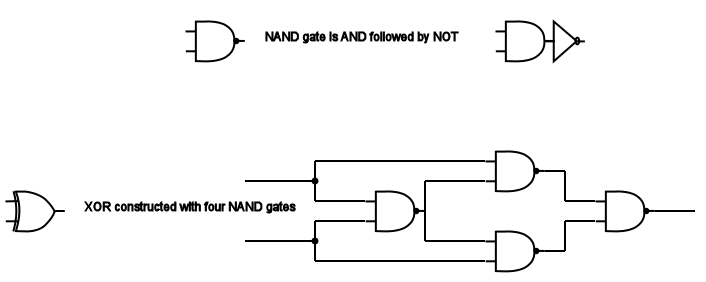
\includegraphics[width=450px]{red6.png}
\end{figure}
\begin{figure}[h]
	\centering
		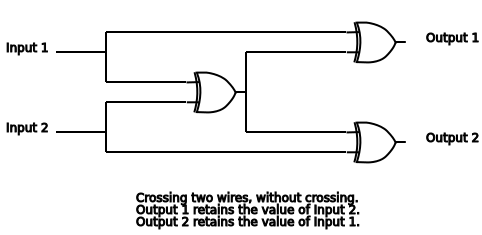
\includegraphics[width=450px]{red6cross.png}
\end{figure}
	\newpage
	\textbf{BOOLCIRCUIT} $\leq$ \textbf{BOOLCIRCUIT2}\\
	Program BOOLCIRCUIT:\\
	\tab Read input $C$.\\
	\tab For each gate $g$ with fanout $>$ 2: \emph{This is done in O($n$) time}\\
	\tabb Replace $g$ with the circuitry described in the following figure.\\
	\tab Output BOOLCIRCUIT2($C$).\\
\begin{figure}[h]
	\centering
		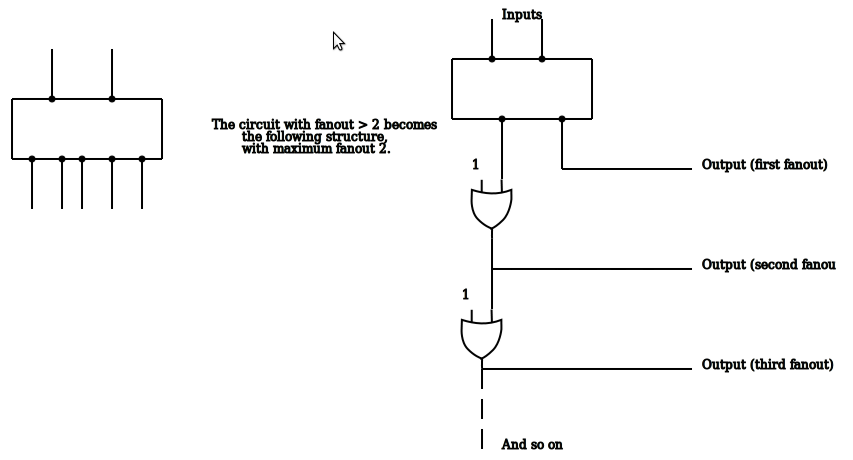
\includegraphics[width=450px]{red6fanout.png}
\end{figure}
	\\
	\textbf{PLANAR} $\leq$ \textbf{BOOLCIRCUIT2}\\
	Program PLANAR:\\
	\tab Read input $C$.\\
	\tab For each gate $g$ with fanout $>$ 2: \emph{This is done in O($n$) time}\\
	\tabb Replace $g$ with the circuitry described in the previous figure.\\
	\tab Output BOOLCIRCUIT2($C$).\\
	\\
    \newpage
	10.		Show that the clique problem is self-reducible.  The decision problem is to take a graph $G$ and an
				integer $k$ and decide if $G$ has a clique of size $k$ or not. The optimization problem takes a graph $G$, and
				returns a largest clique in $G$.  So you must show that if the decision problem has a polynomial time
				algorithm then the optimization problem also has a polynomial time algorithm. Recall that a clique is
				a collection of mutually adjacent vertices.
	\\
	\\
	\textbf{CLIQUE-OPT} $\leq$ \textbf{CLIQUE-DEC}\\
	\\
	Program CLIQUE-OPT:\\
	\tab Read graph $G$, integer $k$.\\
	\tab \emph{First, find the maximum size of the maximum clique.}\\
	\tab For $i$ = $n$ to 1:\\
	\tabb If CLIQUE-DEC($G$,$i$) returns true:\\
	\tabbb size $s$ = $i$.\\
	\tabbb End for-loop.\\
	\tab \emph{Next, find the actual clique by removing the vertices NOT in the clique}\\
	\tab For each vertex $v$ in $G$:\\
	\tab  $G^\prime$ = $G$ - $v$\\
	\tabb If CLIQUE-DEC($G^\prime$, $s$) returns true:\\
	\tabbb $G$ = $G^\prime$.\\
	\tab \emph{G is the graph containing only the maximum-size clique.}\\
	\tab Return $G$.\\
	\newpage
	15.	Consider the following variant of the MST problem. The input consists of an undirected graph $G$ and
			an integer $k$. The problem is to find a spanning tree $T$ of $G$ such that the degree of each node in $T$ is
			at most $k$, or report that no such tree exists. Show by reduction that if this problem has a polynomial
			time algorithm then the Hamiltonian path problem has a polynomial time algorithm. The Hamiltonian
			path problem asks you to determine whether a graph has a simple path that spans the vertices.
	\\
	\\
	\textbf{HAMPATH} $\leq$ \textbf{MST}\\
	\\
	Program HAMPATH:\\
	\tab Read $G$.\\
	\tab $T$ = MST($G$,2).\\
	\tab if $T$ contains all vertices of $G$:\\
	\tabb Return $T$.\\
	\tab Return FAILURE.\\
	\\
	If there exists an MST solution of at most 2 then that tree is a Hamiltonian path. 
\end{document}
